% $Id: chapter1.tex 1790 2010-09-28 16:46:40Z jabriffa $

\chapter{Introduction}

\section{Dissertation Format}
This template is provided to facilitate the process of writing up your
dissertation while ensuring its format is consistent with requirements.
In using this template, \emph{do not}, under any circumstances, make any
changes to the class file provided.
In particular, do not attempt to make any changes to the title page, the
statement of originality, or the copyright page.

Use of this template is not mandatory; if you choose not to use it, then you
must make your final layout resemble this output as closely as possible.
In particular, the textual content and layout of the title page, statement of
originality, and copyright page must not be changed.

\section{Using \LaTeX{}}

\subsection{Supported platform}
The supported platform for this template is a system with:
\begin{itemize}
\item An Ubuntu 10.04 operating system
\item The \verb|texlive-full| package installed
\end{itemize}
This setup is available at least in the Duck/Swan labs, and is supported by
FEPS IT.
The template itself is kept as simple as possible, to facilitate its use on
other systems.

The template also assumes the installation of the GNU make system.
To compile the template into a PDF, simply issue the \verb|make| command
in the template folder, from a terminal.

\subsection{Adding figures}
The simplest way to add figures is to use the \verb|graphicx| package, as shown
in the example that produces Figure~\ref{fig:sample}.
\LaTeX{} automatically finds a suitable place to lay out the figure.
A number of graphic formats are supported -- please refer to the package
documentation for further details.

\begin{figure}[tp]
   \begin{center}
      \subfigure[Diagrammatic representation]{
         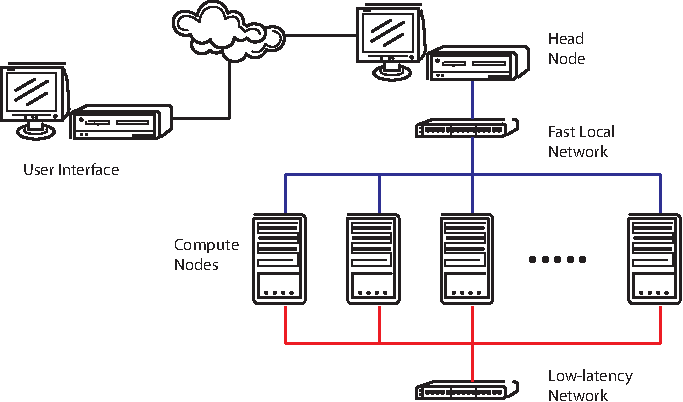
\includegraphics{Figures/cluster}
         }
      \subfigure[Photo of the Tempest cluster]{
         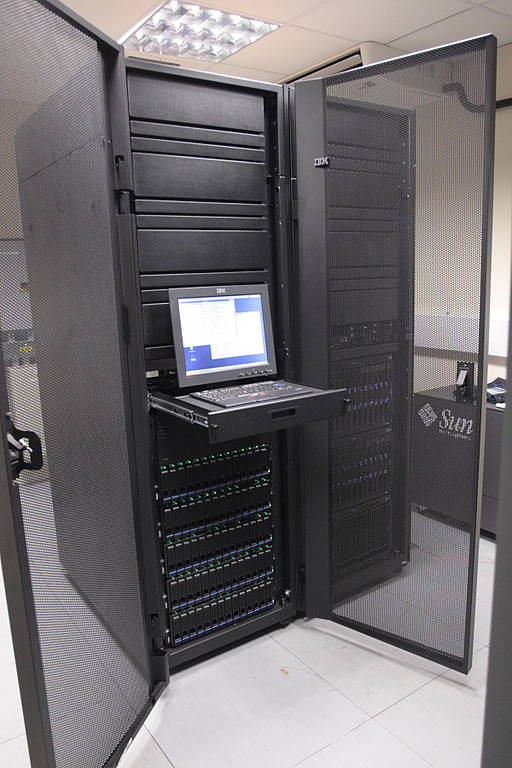
\includegraphics{Figures/tempest}
         }
   \end{center}
   \caption{An example figure, with two parts}
   \label{fig:sample}
\end{figure}

\subsection{Adding tables}
Tables are handled in a similar way to figures, although in this case the text
is entered directly in the source file.
An example is given in Table~\ref{tab:sample}.

\begin{table}[tp]
   \begin{minipage}{\textwidth}
      \begin{center}
         \begin{tabular}{l|c}
            Operation            & Speed \\
            \hline
            Add, Mul, Mul-Add    & 8 \\
            Reciprocal           & 2 \\
            Divide               & 0.88 \\
            Divide Intrinsic     & 1.6 \\
            \hline
            Recip.\ Square Root  & 2 \\
            Square Root          & 1 \\
            \hline
            Logarithm            & 2 \\
            Exponent             & 1 \\
            \hline
            Sin, Cos Intrinsics  & 2 \\
            Sin, Cos, Tan        & Slow \\
         \end{tabular}
      \end{center}
   \end{minipage}
   \caption{An example table, showing speed in operations per cycle per
   multiprocessor}
   \label{tab:sample}
\end{table}
  
\subsection{Adding equations}
One of the strong points of \LaTeX{} is its formatting of mathematical notation.
It can easily handle numbered equations, as in the recursive formula:
\begin{equation}
\alpha(\iota,x_2) = \sum_{x_1,d_{\iota-1}} \alpha(\iota-1,x_1)
   \prob{ \vec{r}_{n(\iota-1)+x_1,n\iota+x_2}, \vec{t}_{\iota-1} }
\end{equation}
or math within the main body of text, for example to specify $1 \leq \iota
< N$.
More complex equations are also handled with ease, as in the following case,
where the equation is too long to fit in a single line:
\begin{equation}
\prob{\vec{r}_{0,n\iota+x_2}, \varsigma_{n\iota}=x_2}
= \sum_{x_1,d_{\iota-1}} \left[
\begin{split}
   & \prob{\vec{r}_{0,n(\iota-1)+x_1}, \varsigma_{n(\iota-1)}=x_1} \\
   & \times \prob{ \vec{r}_{n(\iota-1)+x_1,n\iota+x_2}, \vec{t}_{\iota-1} }
\end{split} \right]
\end{equation}

\subsection{Adding code fragments}
Code fragments in \LaTeX{} can be added using the \verb|verbatim| environment,
as shown in the example below.
Remember to set the line spacing as shown, or you'll end up with double-spaced
code listings.

\singlespaced
\begin{verbatim}
typedef int v4si __attribute__ ((vector_size (16)));

void ArrayAdd(int *c, const int *a, const int *b, int n)
   {
   const v4si *va = (const v4si *)a;
   const v4si *vb = (const v4si *)b;
   v4si *vc = (v4si *)c;
   int i = 0;
   if(n > 4)
      for(; i < n / 4; i++)
         vc[i] = va[i] + vb[i];
   for(i *= 4; i < n; i++)
      c[i] = a[i] + b[i];
   }
\end{verbatim}
\doublespaced

\subsection{Adding references}
One of the more convenient facilities provided by \LaTeX{} is the handling of
references using \BibTeX.
This allows you to completely separate the bibliography database from the
citations within the text, and more importantly from the way these are
formatted.
\BibTeX support a number of reference types; examples are given in this
template for:
\begin{itemize}
\item Conference papers \cite{bsw10icc}
\item Journal articles \cite{gamal}
\item Dissertations \cite{tunstall}
\item Books \cite{press}
\item User or technical manuals \cite{cuda-pg,netpbm}
\item Technical Reports \cite{bw1994}
\item Other material that cannot be easily classified \cite{farrell}
\end{itemize}
